\documentclass[12pt,letterpaper]{article}

% Image support with PDF conversion
\usepackage[pdftex]{graphicx}
% Inserts a line feed between paragraphs, because it makes me feel grown up
\usepackage{parskip}
% Underline text using \uline{...}
\usepackage[normalem]{ulem}
% Sane URL handling
\usepackage{url}
% Math equations
\usepackage{mathtools}
% source code typesetting
\usepackage{algpseudocode}
\usepackage{listings}
% Implement the ARRL's oddly specific margin and page number equirements
\usepackage[top=0.8in, bottom=1in, left=0.75in, right=0.75in]{geometry}
\pagenumbering{gobble}


\title{Clarifying Amateur Bell 202}

\author{Kenneth Finnegan, W6KWF\\
\small Masters Student, Electrical Engineering Department\\
\small California Polytechnic State University, San Luis Obispo\\
\small \texttt{http://blog.thelifeofkenneth.com/}\\
\small \texttt{kennethfinnegan2007@gmail.com}\\
\and
Bridget Benson, Ph.D.\\
\small Assistant Professor, Electrical Engineering Department\\
\small California Polytechnic State University, San Luis Obispo\\
\small \texttt{http://www.calpoly.edu/\textasciitilde{}bbenson/}\\
\small \texttt{bbenson@calpoly.edu}}


\begin{document}
\maketitle

\begin{abstract}
	Since its inception more than three decades ago, 
	packet radio has seen several huge changes in technology
	and applications. 
	Despite its age, the 1200 baud Bell 202 modulation used in some
	of the earliest packet systems still enjoys a wide user base
	in several of the major packet networks still in operation.
	Oddly, despite being one of the longest-lived amateur packet modulations in use,
	the amateur community seems to have neglected to ever write a detailed
	specification document for this integral part of so many packet systems.
	This paper curates the information garnered from countless sources
	in the hopes that other amateurs developing modems for 
	this prototypical modulation
	don't need to follow the author in spending such an inordinate amount of
	time and energy researching and reverse-engineering what should be a
	well-established specification.
	
	
	\textbf{Keywords:} AFSK, AX.25, Bell 202, Packet Radio, Specification
\end{abstract}


\section{Bell 202 in Amateur Radio}
\label{sec:bell202history}

Bell 202 is an audio frequency shift keyed (AFSK) modulation that
encodes data by shifting between 1200Hz and 2200Hz audio tones.
These tones respectively represent a binary one or zero and transitions happen
at a rate of 1200 symbols per second.
Originally developed by AT\&T for use on the telephone network \cite{202tspec},
Bell 202 was selected for amateur radio packet operations due to the abundance
of modems available on the second-hand market in 1981 when the FCC authorized
amateur packet operations in the United States \cite{gatewaypacket}.

\begin{figure}
	\centering
	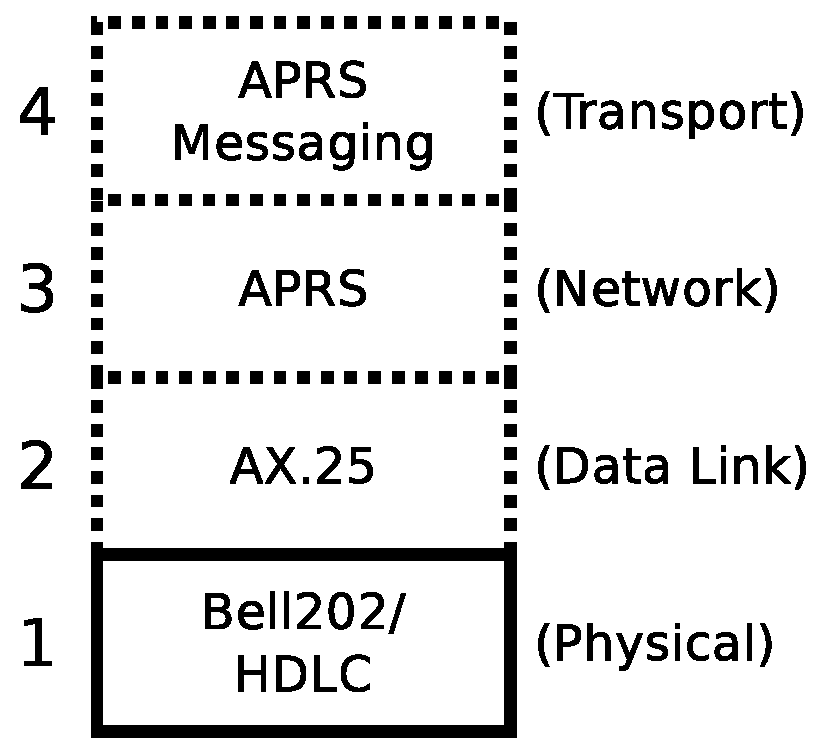
\includegraphics[width=0.4\textwidth]{src/dia/osi_bell202}
	\caption{OSI network layers for a typical packet radio application}
	\label{fig:osibell}
\end{figure}

Like most real-world network protocols, there isn't a particularly clean
mapping of packet radio protocols to the seven layers of the OSI
network model. To help clarify references to the different layers in this article,
figure \ref{fig:osibell} shows an example of Bell 202 as used in the APRS
network stack.
Due to Amateur radio operators
using Bell 202 as a physical layer below AX.25, which is a derivative of
X.25, the physical layer implicitly includes the High-Level Data Link Control (HDLC) 
protocol for framing and bit stuffing \cite{n1vgphy}.
This means that the original 1200Hz mark and 2200Hz space symbols
do not directly represent one and zero;
the AX.25 data stream is encoded using the 
inverted non-return to zero (NRZI) encoding,
which calls for zeros in the original bit stream to be encoded as a change
between 1200Hz and 2200Hz and ones to be encoded as transmitting the same
tone during two consecutive symbol periods \cite{iso13239}.

\section{Bell 202 Transmission Format}

\begin{figure}
	\centering
	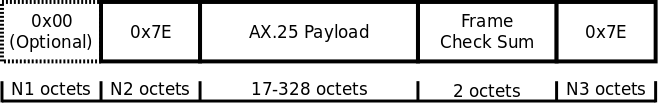
\includegraphics[width=1.0\textwidth]{src/dia/bell202}
	\caption{Bell 202/HDLC frame format}
	\label{fig:bell202format}
\end{figure}

Figure \ref{fig:bell202format} shows the format of a typical single frame
Bell 202 transmission. There are a number of important facets to note:
\begin{itemize}
	\item The leading 0x00 octets are mentioned in very few documents
		discussing Bell 202, yet they reportedly improve modem
		throughput \cite{millerinterview}\cite{aprsunveiled}. 
		0x00 encoded in NRZI causes a symbol transition
		every clock cycle and thus provides a more effective clock 
		synchronization target than the originally specified 0x7E octets. 
		0x7E is actually 
		the longest allowable string of 1s in the frame and 
		therefore has the lowest amount of energy at the clocking frequency,
		which causes it to be the \emph{worst} 
		octet for asynchronous clock recovery.
	\item The octet 0x7E is used to indicate the beginning and end of 
		Bell 202 / HDLC frames.
		There is little guidance on the number of flag octets before
		or after frames (represented by N2 and N3 in 
		figure \ref{fig:bell202format})
		beyond stating that there must be at least one of each. The sum of
		N1 and N2 is variable in most modems via the ``TXDelay" parameter,
		which specifies how long the preamble is in 10ms increments.
	\item It is permissible to encode multiple 
		frames per transmission, yet there is no guidance as to how
		many octets of 0x7E be included between them.
		Most modems insert several 0x7E octets between 
		frames.\footnote{For a specific example, the Argent Data OT3m TNC 
			with firmware r56474 inserts 3 flags before
		a frame, 7 flags between two frames, and 5 flags after the final frame.}
		Tests indicate that the number of flags between frames 
		impact throughput of the following frame, yet
		quantitative measurements of this effect proved elusive.
	\item The frame payload and frame check sum must be bit stuffed such 
		that no string of more than five 1's appear in a row.
		This is done by ``bit-stuffing" the transmitted bitsteam by
		appending a zero after any string of five ones at the transmitter,
		and subsequently dropping this zero following five ones at the 
		receiver.\footnote{Six ones in a row represent a 0x7E flag indicating 
			the end of a frame or an idle carrier.
			Seven or more ones in a row indicate an invalid channel state
			that shouldn't happen, but regularly does, so modems must be 
			able to handle arbitrary strings of ones gracefully.}
	\item Every octet is encoded and transmitted least significant bit first,
		except for the CRC-16-CCITT Frame Check Sum, 
		which is transmitted big-endian
		and most significant big first.
		\cite{n1vgphy},\cite[\S8.1.1-2]{ituv42},\cite[\S3.8]{ax25spec}.
		See section \ref{calcfcs} for further discussion.
	\item The minimum and maximum payload sizes indicated in figure 
		\ref{fig:bell202format} aren't enforced by any properties of 
		Bell 202 or HDLC, but from the Maximum Transmission Unit (MTU)
		specified in the AX.25 network stack.
		Larger frames are possible, and were often used in specialized 
		AX.25 and IPv4 packet networks \cite{pattersoninterview}.

\end{itemize}

\subsection{Excluding HDLC from AX.25 layer 2}

It is important to note that the presentation of the HDLC framing
and checksum
in figure \ref{fig:bell202format} as part of the layer 1 modulation 
instead of as part of the layer 2 AX.25 frame is 
novel to this work and hasn't been seen in any of the existing literature.
This change was made because including the frame checksum and flags
in the layer 2 documentation confuses the separation between Bell 202 
and AX.25. 

This is particularly important when AX.25 packets are transfers across 
other layer 1 links with their own framing protocols.
The KISS serial link between a host system and modem is the most notable
transport where these fields are not included and post-facto generated by the
Bell 202 modem during transmission \cite{KISSspec}.
M. Chepponis and P. Karn made the technically correct decision of excluding 
HDLC framing from the binary payload when developing KISS, but this caused
an unfortunate situation where KISS is transporting an entirely
undocumented fragment of the AX.25 packet. Figure \ref{fig:ax25format} 
shows what the AX.25 layer 2 should be presented as.

\begin{figure}
	\centering
	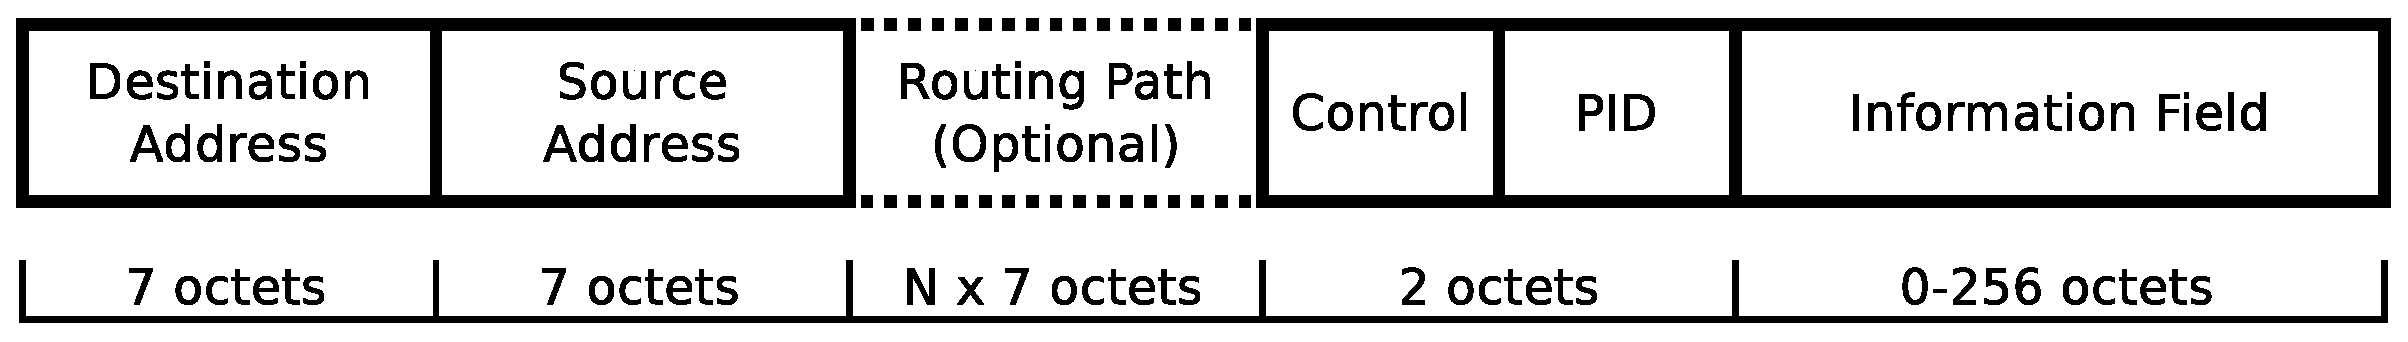
\includegraphics[width=1.0\textwidth]{src/dia/ax25}
	\caption{Modified AX.25 packet format excluding HDLC fields.}
	\label{fig:ax25format}
\end{figure}

\subsection{Calculating the Frame Check Sum}
\label{calcfcs}


The CRC used for error detection is the well-known CRC-16-CCITT, which
enjoys a wide deployment in network protocols and 
systems\footnote{Example systems include HDLC, Bluetooth, the XMODEM file 
transfer protocol, and SD cards}.
Unfortunately, the language used in \S4.2.5 of the ISO specification for
HDLC \cite{iso13239} is particularly awkward, 
and doesn't lend itself well to implementation.
For the sake of clarity, figure \ref{fig:crcccittcode} 
presents one possible algorithm to
calculate the CRC checksum of a complete frame.
The constant 0x8408 comes from a bit reversal of the 0x1021 generator polynomial
since the presented algorithm calculates the CRC in bit reversed order.

The order of the two octets and bit order of the checksum 
as transmitted over the air 
is particularly muddled in the existing amateur literature, 
since many amateur sources call for sending the
checksum little-endian, while ITU V.42 \S8.1.2.3 specifies big-endian,
as is the convention for most network protocols.
The original specifications also call for transmitting the checksum most
significant bit (MSb) first, which is the opposite of the payload octets.
This exception is noted in \S3.8 of the AX.25 specification, 
but never appears to be handled by most implementations\footnote{Examples
include TNC-X and APRX.}.

This confusion likely comes from the fact that most amateurs are copying
available reference implementations of the CRC checksum such as
figure \ref{fig:crcccittcode} that,
unbeknownst to the amateur, already integrate the called for bit reversal 
after the CRC division and one's complement.
The algorithm presented \emph{does not} calculate the true CCITT CRC checksum, but
calculates it in reverse bit order such that the final bit-reversal step 
can be neglected during modulation of the bit stream.
Therefore, the checksum as presented should be sent lower octet first, 
using the same modulator as the payload octets that modulates the LSb first.
This ensures that the resulting checksum as transmitted will have the 
correct sequence, starting with the MSb and finishing with the LSb.


\begin{figure}
	\begin{algorithmic}[1]
		\Function{calculate\_crc}{$frame[~], frame\_length$}
		\State $crc \gets \texttt{0xFFFF}$

		\ForAll{$byte \gets frame_{0}, frame_{frame\_length-1}$}
		\ForAll {$bit \gets byte_{LSb}, byte_{MSb}$}
		\If {$crc_{LSb} \neq bit$}
			\State $crc \gets (crc \gg 1) \textrm{ XOR } \texttt{0x8408}$
			%\Comment{Right shift and XOR with bit-reversed polynomial}
		\Else
			\State $crc \gets crc \gg 1$
			%\Comment{Only right shift}
		\EndIf
		\EndFor
		\EndFor

		\State $crc \gets crc \textrm{ XOR } \texttt{0xFFFF}$
		%\Comment{Take one's complement per ITU-T V.42 \S8.1.1.6.2}

		%\Comment{Swap high and low bytes so crc is in host endian order}
		\State \textbf{return} $crc$
		\EndFunction
	\end{algorithmic}

	\caption{Algorithm to calculate CRC-16-CCITT in reverse-bit order.}
	\label{fig:crcccittcode}
\end{figure}

\section{FM Deviation and Emphasis}

Once the HDLC frame is generated, encoded using NRZI, and converted into
a baseband AFSK signal, it still needs to be converted into a VHF FM signal
and transmitted to other stations. 
Since Bell 202 was originally designed for telephone data service, 
the existing specifications give absolutely no guidance on the unique 
aspects of the amateur VHF FM physical layer, such as what 
FM deviation to target when setting modem audio levels.

While quantitatively justifying this figure is beyond the ability of the
author, a proposed specification for FM deviation is 3.5kHz for both
1200Hz and 2200Hz tones, or for the wider of the two tones if equal
deviation is not possible \cite{millerinterview}.

This proposal is complicated by two major issues: 
\begin{itemize}
	\item The lack of availability of the necessary 
		test equipment to measure FM deviation.
	\item The inconsistency in pre-emphasis and de-emphasis filters
		used by individual network nodes.
\end{itemize}

The VHF service monitor needed to properly set modem deviation is prohibitively
expensive for the typical packet radio operator, so presenting a figure 
such as 3.5kHz deviation to most users makes little difference.
Qualitative and home-brew solutions have been developed
for setting deviation levels\cite{n8urdev},
and these techniques should be better promoted until 
deviation meters become a more standard part of a packet operator's toolkit. 

\begin{figure}
	\centering
	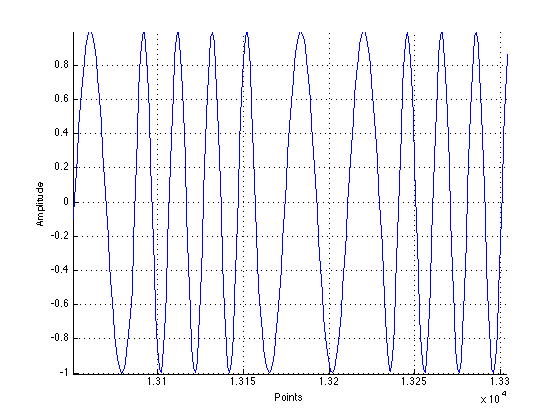
\includegraphics[width=0.7\textwidth]{src/bell202sample}
	\caption{Typical Bell 202 baseband signal}
	\label{fig:bell202sample}
\end{figure}

Pre-emphasis and de-emphasis is a concept in FM voice communications where
higher baseband frequencies are more widely modulated than lower ones
to provide a consistent signal to noise ratio across the channel.
Unfortunately, the advantage of these audio filters to packet operation 
are debatable, and they are not applied consistently. A given packet 
station is likely to have any permutation of pre-emphasized or flat 
transmit audio and de-emphasized or flat receive audio.
This means that even when one station deliberately uses flat audio,
there is no guarantee that it won't suffer from receiving another
station's pre-emphasized signal or be received by another station using de-emphasis.

Different types of Bell 202 modems vary in how sensitive they are to this high/low
pass filtering effect, but more importantly there is no benchmark established
for what level of pre-/de-emphasis a modem should tolerate.
One suitable source for such a benchmark would be to go back to the
telephone networks where Bell 202 was originally used.
Figure \ref{fig:3002} shows the allowable audio distortion of a basic type 3002
channel as used in the telephone network; any level of distortion that falls 
inside the shaded region relative to a test tone at 1004 Hz is considered acceptable.

For application to amateur Bell 202, the distortion figures normalized to 1004Hz is 
less critical than the fact that the allowable distortion between the two
tones of interest (1200Hz and 2200Hz) is 10dB in either direction.
An insightful measurement for Bell 202 modem designers would be testing how
quickly their modem's performance falls off as packet signal approaches these limits.
Designing and making available a test suite which could yield quantitative
measures of a modem's sensitivity to the pre-emphasis/de-emphasis issue would
be a work beyond the scope of this paper that would be of great value.

\begin{figure}
	\centering
	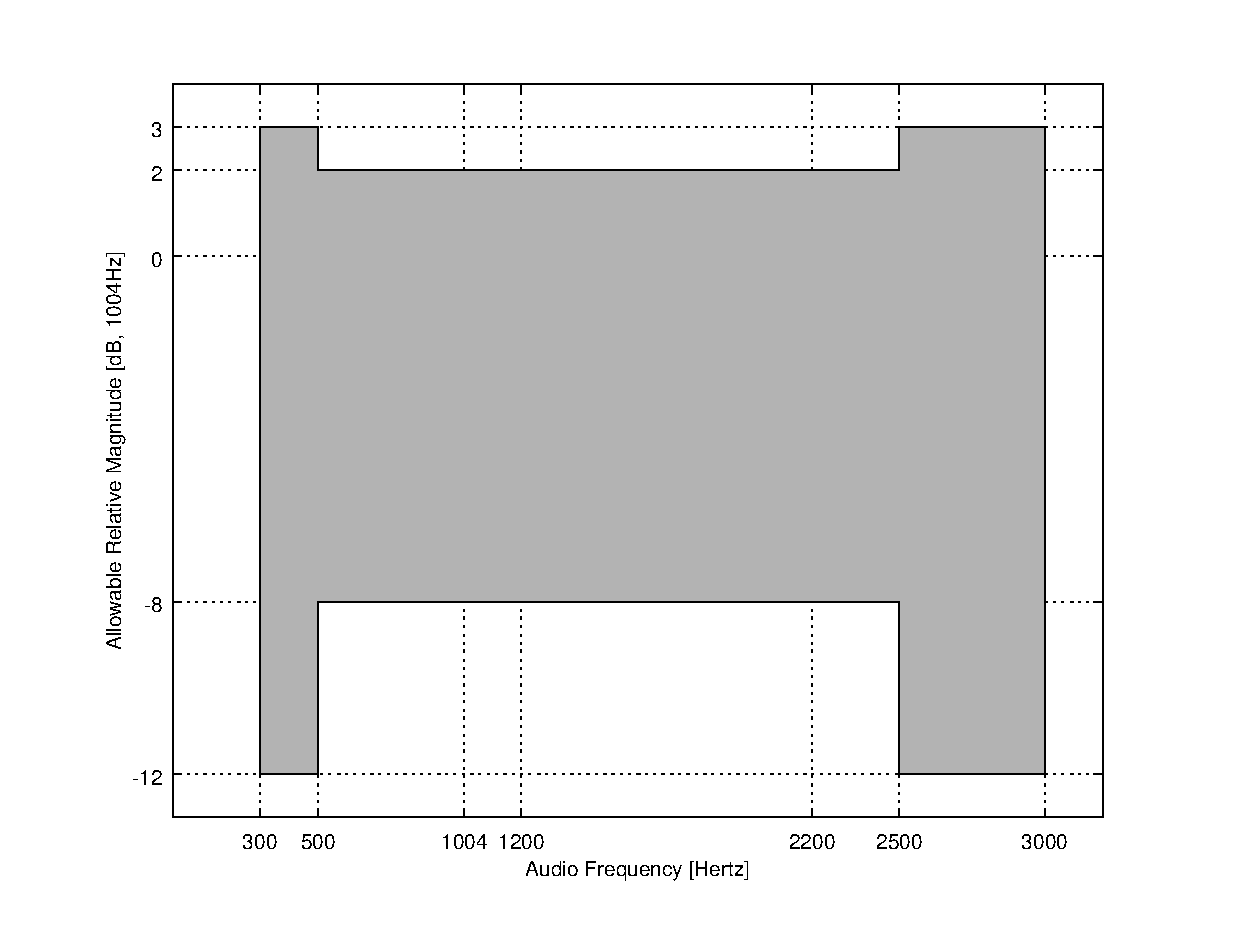
\includegraphics[width=0.7\textwidth]{src/octave/3002}
	\caption{Allowable distortion in a basic 3002 telephone channel}
	\label{fig:3002}
\end{figure}


\section{Carrier Sense Multiple Access}
\label{sec:bell202csma}

Since amateur Bell 202 is a half duplex modulation using re-purposed 
FM voice transceivers, 
one of the challenges to packet radio is avoiding multiple stations
transmitting on the same channel at once. 
Other derivatives of ALOHAnet, 
such as half duplex 10Mbps Ethernet, 
enjoy the advantage that transmitters can
at least sense when a collision has taken place 
and use that information to abort the transmission of the rest of the frame.

Besides the degenerate case of ignoring the current channel status completely when 
deciding to transmit a pending frame\footnote{This is a surprisingly
	common channel access method, used primarily by what are called ``dumb" or
	``deaf" APRS trackers, which are transmit-only and entirely lack an
FM receiver altogether.}, there are two popular algorithms used for
channel access in North America;
DWait and P-persistent.

DWait is a deterministic algorithm where each station is assigned a fixed
``quiet time" after the end of any other transmission 
before they will begin a locally pending transmission. 
This lends itself well to designed networks
where the relative priority of each station is known and a corresponding DWait time
is set for each station where a shorter DWait will 
always gain the channel over a longer one. 
Conversely, this doesn't lend itself well to ad-hoc networks, since
two stations that happen to end up near one another with similar DWait parameters
and pending traffic will tend to collide and hurt throughput.

P-persistent is a stochastic algorithm that attempts to fairly spread
stations apart when the channel becomes clear. 
This is configured with two variables: the slot time (SLottime), and the
probability that a station should choose to transmit during a given slot (PErsist). 
The SLottime
should be set to as short of a time interval as possible during which a station can
reliably identify another station as transmitting 
before beginning its own transmission.
The PErsist value should be tuned based on how likely another station is to transmit 
considering the number of other stations with 
pending traffic attempting to gain the channel.

A typical modem supporting the p-persist algorithm will need three values adjusted
based on the specific network hardware in use; PErsist, SLottime, and the 
transmitter preamble time TXDelay mentioned earlier in this paper.

\begin{itemize}
	\item PErsist: Measured in units of 1/256, the suggested default is
		63, which translates into a 0.25 chance of selecting a specific available
		slot. A typical implementation selects random number in the range
		[0,255] and tests if it is equal or less than the PErsist value.
		Therefore, a setting of 0 would result in a 0.004 chance of selecting 
		a slot and a setting of 255 would result in always selecting a slot.
		The optimal value for a specific network is highly dependent on the
		local channel occupancy, so the suggested default shouldn't
		be considered definitive.
	\item SLottime: Measured in units of 10ms increments, the traditional
		default from sources such as the KISS specification and 
		Kantronics hardware is a value of 10 (100ms), 
		but performance measurements of contemporary VHF radios 
		indicate a need for a longer slot time. 
		The new suggested value is 30 (300ms).
	\item TXDelay: Measured in units of 10ms increments, the suggested
		default is a value of 50, which translates into a 500ms synchronization
		preamble from when a transmitter is keyed up until when a payload
		frame is transmitted.
		This value is very conservative and can usually be reduced when
		receiving stations are properly configured with
		well aligned clock recovery mechanisms.
\end{itemize}

TODO: Say something about DAMA?

\section{Conclusion}


By most measures, Bell 202 is a very poor performing modulation to
be used by amateurs for packet operations. 
One bit symbols cause Bell 202 to suffer from poor spectral efficiency,
HDLC lacks any error correcting codes so single bit errors cause entire 
frames to be dropped, and 1200 bits per second is an almost laughably slow
data rate when even consumer radio systems are operating at hundreds of millions
of bits per second throughput.

One property of Bell 202 that is appealing, other than the 
huge legacy systems still using it, is it's relative simplicity.
The fact that amateurs are able to implement Bell 202 modems on
systems as minimalistic as 8 bit microcontrollers, and these modems can 
interface with standard voice radios without requiring internal modification, 
make Bell 202 much more accessible than more sophisticated modulations.

Faster data rates and more sophisticated modems should never be discouraged,
but the value of being able to learn about amateur digital communications 
via the simplicity of Bell 202 can't be discounted.
Unfortunately, as the technological landscape where 
protocols such as Bell 202 or AX.25 were developed in moves further into the past,
the need to write additional documentation that gives sufficient context to 
the next generation of packet radio operators is going to become increasingly 
critical to the digital communications aspect of the amateur radio hobby.


\appendix
\section{SLottime Justification}
\label{vhftxrx}

The SLottime parameter of modems is dependent upon the total time
it takes for one station to begin transmitting and for receiving stations
to subsequently identify the channel as occupied.
This sequence can be broken into the following stages:
\begin{itemize}
	\item Transmitter key-up from standby (RX-TX turnaround time)
	\item RF propagation from transmitter to receiver (negligible)
	\item Receiver opening squelch and outputting AFSK signal to modem. 
		(While not usually measured, a representative measurement is
		the TX-RX turnaround time)
	\item Modem Data Carrier Detect (DCD) of the received signal
\end{itemize}

Since most Bell 202 packet activity is done using amateur VHF mobile radios,
a survey was performed of every ARRL QST hardware review published on VHF-capable
mobile radios since 1999.

TODO: Table of collected values.





\begin{thebibliography}{99}

	\bibitem{TODO}
		TODO: Sort citations

	\bibitem{millerinterview}
		S. Miller. Personal interview. 25 Mar. 2014.

	\bibitem{ax25spec}
		W. Beech, et al.,
		\emph{AX.25 Link Access Protocol for Amateur Packet Radio Version 2.2}.
		Tucson, Arizona: Tucson Amateur Packet Radio Corp, 1998. 
		\url{http://www.tapr.org/pdf/AX25.2.2.pdf}

	\bibitem{iso13239}
		\emph{Information technology --- Telecommunications and information
			exchange between systems --- High-level data link control (HDLC)
		procedures}, ISO Standard 13239, 2002.

	\bibitem{202tspec}
		American Telephone and Telegraph Company,
		\emph{Data Sets 202S and 202T Interface Specification},
		AT\&T Publication 41212,
		July, 1976.

	\bibitem{KISSspec}
		M. Chepponis, P. Karn,
		``The KISS TNC: A simple Host-to-TNC communications protocol,"
		in \emph{ARRL 6th Computer Networking Conference},
		1987, pp/~38-43.
		Translated to HTML Jan. 1997 by P. Karn,
		\url{http://ax25.net/kiss.aspx}

	\bibitem{n1vgphy}
		S. Miller,
		``1200 Baud Packet Radio Details."
		\url{http://n1vg.net/packet/index.php}

	\bibitem{aprsunveiled}
		B. Simmons,
		``APRS Unveiled," in \emph{QEX},
		pp.~19-23,
		Nov./Dec. 2012.

	\bibitem{ituv42}
		\emph{Error-correcting procedures for DCEs using 
		asynchronous-to-synchronous conversion}, ITU-T standard V.42, 2002.

	\bibitem{n8urdev}
		J. Ackermann,
		``Setting Your TNC's Audio Drive Level."
		\url{http://www.febo.com/packet/layer-one/transmit.html}

	\bibitem{pattersoninterview}
		R. Patterson. Personal interview. 31 Mar. 2014.

	\bibitem{gatewaypacket}
		S. Horzepa,
		\emph{Your Gateway to Packet Radio},
		Newington, Connecticut: American Radio Relay League, 1989.

\end{thebibliography}


\end{document}

